\documentclass[12pt]{gatech-thesis}
\usepackage{amsmath,amssymb,latexsym,float,epsfig,subfigure}
\usepackage{wrapfig}
%% editing comment

%\newcommand{\cmt}[1]{\textcolor{red}{\textbf {#1}}}
\newcommand{\cmt}[1]{}
\newcommand{\note}[1]{\cmt{Note: #1}}
\newcommand{\karen}[1]{\textcolor{red}{{Karen: #1}}}
\newcommand{\john}[1]{\textcolor{cyan}{{John: #1}}}
\newcommand{\sehoon}[1]{\textcolor{magenta}{{Sehoon: #1}}}
\newcommand{\sehoontext}[1]{\textcolor{magenta}{{#1}}}
\newcommand{\newtext}[1]{#1}
\newcommand{\original}[1]{\textcolor{magenta}{Original: #1}}
\newcommand{\updated}[1]{\textcolor{blue}{Updated: #1}}
\newcommand{\revised}[1]{\textcolor{blue}{#1}}

\newcommand{\myparagraph}[1]{\vspace{0.33cm} \noindent \textbf{#1. }}


%% ignore text
\long\def\ignorethis#1{}

%% abbreviations
\newcommand{\etal}{{\em{et~al.}\ }}
\newcommand{\eg}{e.g.\ }
\newcommand{\ie}{i.e.\ }

%% reference shortcuts
\newcommand{\figtodo}[1]{\framebox[0.8\columnwidth]{\rule{0pt}{1in}#1}}
\newcommand{\figref}[1]{Figure~\ref{fig:#1}}
\newcommand{\tabref}[1]{Table~\ref{tab:#1}}
\newcommand{\eqnref}[1]{Equation~(\ref{eq:#1})}
%\renewcommand{\eqref}[1]{Equation~(\ref{eq:#1})}
\newcommand{\secref}[1]{Section~\ref{sec:#1}}

%% frequently used mathematical structures
\newcommand{\vc}[1]{\ensuremath{\mathbf{#1}}}
\newcommand{\pd}[2]{\ensuremath{\frac{\partial{#1}}{\partial{#2}}}}
\newcommand{\pdd}[3]{\ensuremath{\frac{\partial^2{#1}}{\partial{#2}\,\partial{#3}}}}

%% New commands for Sehoon!
\newcommand{\mat}[1]{\ensuremath{\mathbf{#1}}}
\newcommand{\set}[1]{\ensuremath{\mathcal{#1}}}

% math macros
\newcommand{\vEndEff}{\ensuremath{\vc{d}}}
\newcommand{\vRelMove}{\ensuremath{\vc{r}}}
\newcommand{\sSet}{\ensuremath{S}}


\newcommand{\vControl}{\ensuremath{\vc{u}}}
\newcommand{\vPoint}{\ensuremath{\vc{p}}}
\newcommand{\sSpringCoef}{{\ensuremath{k_{s}}}}
\newcommand{\sDamperCoef}{{\ensuremath{k_{d}}}}
\newcommand{\vHandle}{\ensuremath{\vc{h}}}
\newcommand{\vForce}{\ensuremath{\vc{f}}}

\newcommand{\mTransChain}{\ensuremath{\vc{W}}}
\newcommand{\mRotateTrans}{\ensuremath{\vc{R}}}
\newcommand{\sJoint}{\ensuremath{q}}
\newcommand{\vJoint}{\ensuremath{\vc{q}}}
\newcommand{\mJoint}{\ensuremath{\vc{Q}}}
\newcommand{\mMass}{\ensuremath{\vc{M}}}
\newcommand{\sMass}{\ensuremath{{m}}}
\newcommand{\vGravity}{\ensuremath{\vc{g}}}
\newcommand{\vConstr}{\ensuremath{\vc{C}}}
\newcommand{\sConstr}{\ensuremath{C}}
\newcommand{\vCOM}{\ensuremath{\vc{x}}}
\newcommand{\sGeneralForce}[1]{\ensuremath{Q_{#1}}}
\newcommand{\vStateVar}{\ensuremath{\vc{y}}}
\newcommand{\vControlVar}{\ensuremath{\vc{u}}}
\newcommand{\argmax}{\operatornamewithlimits{argmax}}
\newcommand{\argmin}{\operatornamewithlimits{argmin}}
\newcommand{\tr}[1]{\ensuremath{\mathrm{tr}\left(#1\right)}}




%%%%%%%%%%%%%%%%%%%%%%%%%%%%%%%%%%%%%%%%%%%%%%%%%%%%%%%%%%%%%%%%%%%
%
% Here are a bunch of macros, mostly for math.
%
%%%%%%%%%%%%%%%%%%%%%%%%%%%%%%%%%%%%%%%%%%%%%%%%%%%%%%%%%%%%%%%%%%%

\renewcommand{\choose}[2]{\ensuremath{\left(\begin{array}{c} #1 \\ #2 \end{array} \right )}}

\newcommand{\gauss}[3]{\ensuremath{\mathcal{N}(#1 | #2 ; #3)}}

\newcommand{\pctab}{\hspace{0.2in}}
\newenvironment{pseudocode} {\begin{center} \begin{minipage}{\textwidth}
                             \normalsize \vspace{-2\baselineskip} \begin{tabbing}
                             \pctab \= \pctab \= \pctab \= \pctab \=
                             \pctab \= \pctab \= \pctab \= \pctab \= \\}
                            {\end{tabbing} \vspace{-2\baselineskip}
                             \end{minipage} \end{center}}
\newenvironment{items}      {\begin{list}{$\bullet$}
                              {\setlength{\partopsep}{\parskip}
                                \setlength{\parsep}{\parskip}
                                \setlength{\topsep}{0pt}
                                \setlength{\itemsep}{0pt}
                                \settowidth{\labelwidth}{$\bullet$}
                                \setlength{\labelsep}{1ex}
                                \setlength{\leftmargin}{\labelwidth}
                                \addtolength{\leftmargin}{\labelsep}
                                }
                              }
                            {\end{list}}
\newcommand{\newfun}[3]{\noindent\vspace{0pt}\fbox{\begin{minipage}{3.3truein}\vspace{#1}~ {#3}~\vspace{12pt}\end{minipage}}\vspace{#2}}



\newcommand{\key}{\textbf}
\newcommand{\fun}{\textsc}

\newcommand{\mytilde}{\raise.17ex\hbox{$\scriptstyle\mathtt{\sim}$}}

%\def\shortcite{\def\citename##1{}\@internalcite}

% Local Variables:
% TeX-master: "paper"
% End:


%%
%% This example is adapted from ucthesis.tex, a part of the
%% UCTHESIS class package...
%%
\title{Learning Dynamic Motor Skills \protect\\
  for Virtual and Real Humanoids} 
%% If you want to specify a linebreak
                               %% in the thesis title, you MUST use
                               %% \protect\\ instead of \\, as \\ is a
                               %% fragile command that \MakeUpperCase
                               %% will break!
\author{Sehoon Ha}
\department{School of Computer Science}

%% Can have up to six readers, plus principaladvisor and
%% committeechair. All have the form
%%
%%  \reader{Name}[Department][Institution]
%%
%% The second and third arguments are optional, but if you wish to
%% supply the third, you must supply the second. Department defaults
%% to the department defined above and Institution defaults to Georgia
%% Institute of Technology.

\principaladvisor{Professor C. Karen Liu}
\firstreader{Professor Greg Turk}
\secondreader{Professor Jarek Rossignac}
\thirdreader{Professor Jun Ueda}[School of Mechanical Engineering]
\fourthreader{Professor Katsu Yamane}[Disney Research Pittsburgh][]
\degree{Doctor of Philosophy}

%% Set \listmajortrue below, then uncomment and set this for
%% interdisciplinary PhD programs so that the title page says
%% ``[degree] in [major]'' and puts the department at the bottom of
%% the page, rather than saying ``[degree] in the [department]''

%% \major{Algorithms, Combinatorics, and Optimization} 

\copyrightyear{2015}
\submitdate{December 2015} % Must be the month and year of graduation,
                         % not thesis approval! As of 2010, this means
                         % this text must be May, August, or December
                         % followed by the year.

%% The date the last committee member signs the thesis form. Printed
%% on the approval page.
\approveddate{14 August 2015}

%% \bibfiles{example-thesis}
\bibfiles{thesis}

%% The following are the defaults
%%    \titlepagetrue
%%    \signaturepagetrue
%%    \copyrightfalse
%%    \figurespagetrue
%%    \tablespagetrue
%%    \contentspagetrue
%%    \dedicationheadingfalse
%%    \bibpagetrue
%%    \thesisproposalfalse
%%    \strictmarginstrue
%%    \dissertationfalse
%%    \listmajorfalse
%%    \multivolumefalse

\begin{document}
\bibliographystyle{gatech-thesis}
%%
\begin{preliminary}
\begin{dedication}
\null\vfil
{\large
\begin{center}
To myself,\\\vspace{12pt}
Sehoon Ha,\\\vspace{12pt}
the only person worthy of my company.
\end{center}}
\vfil\null
\end{dedication}
%% \begin{preface}
%% Theses have elements.  Isn't that nice?
%% \end{preface}
\begin{acknowledgements}
I cannot begin to express my thanks to my wife, Jennifer Gahee Kim,
who sincerely supports me with love, wisdom, insight, and delicious foods.
It is very special to share my life with someone who is not just my wonderful
wife, but also the greatest friend a person could ever have.
You make my life happier than ever.

I also want to thank my mother Jiwon and my father Sangsoo for guiding me
throughout my life.
I would not have been able to find, start, and finish the graduate school without
their unconditional love and support.

I am also grateful to my brother Jihoon, his family Eunchae and Dongkwon,
and parents-in-law Eungyoung Lee and Boogyun Kim for encouraging me to pursuit
my degree.
Especially, my brother has been a great tutor who teaches me
how to add numbers, how to program, how to solve puzzles, and many more
in the most interesting ways.

I want to thank the members of my committee: Greg Turk, Jarek Rossignac,
Jun Ueda, Katsu Yamane, and my advisor C. Karen Liu.
Each of you encouraged and help me to become a much stronger and solid
researcher with insightful suggestions on my research direction and
communication skills.

I would like to extend my sincere thanks to my labmates
who have shared invaluable discussions during the entire program:
a co-advisor Yuting Ye, Jie Tan, Yunfei Bai, Karthik Raveendran, 
Sumit Jain, Yuting Gu, Chen Tang, John Turner, Alex Clegg, Kihwan Kim, 
Chirs Wojtan, Jason Williams, Jihun Yu, Tina Zhou, Mark Luffel, 
Topraj Gurung, Kristin Siu, Yunseong Song,
Jeongseok Lee, Wenhao Yu, and many more.
In addition, I would like to thank my old friends/mentors: Yeongjin, Seongmin,and Jaesik.
I am really sorry if I forgot anyone.

I wish to particularly thank Evan Kanso, Jovan Popovi\'{c}, Jim McCann, and
Katsu Yamane, who provided me with encouragement and patience throughout the
duration of my internships: all the experiences widen my research horizons.

Special thanks to my mentors, Wangjae Lee and Jaehong Kim, who
guides my life to the better direction.

I would like to express my deepest appreciation to my advisor, C. Karen Liu.
I feel extremely fortunate to have her as my advisor.
Her intellectual insights and creativity to research problems was a great
source of inspiration which carves me as a better researcher.
Her enthusiasm of research encourages me to keep working on more challenging
problems, which is one of the most valuable lessons learned in my life.
It was a great honor to be under her supervision for the last six years.
I will miss all interactions with you, Karen, 
including both insightful discussions and fun jokes. 













\end{acknowledgements}
% print table of contents, figures and tables here.
\contents
% if you need a "List of Symbols or Abbreviations" look into
% gatech-thesis-gloss.sty.
\begin{summary}
%1234567890123456789012345678901234567890123456789012345678901234567890123456789

Demonstrating strength and agility on virtual and real humanoids has
been an important goal in computer graphics and robotics.
However, developing physics-based controllers for various agile motor skills
requires a tremendous amount of prior knowledge and manual labor due to
complex mechanisms \revised{of motor skills}.
The focus of the dissertation is to develop a set of computational tools to
expedite the design process of physics-based controllers that can execute a
variety of agile motor skills on virtual and real humanoids.
Instead of directly \revised{designing controllers} on real humanoids, this
dissertation takes an approach that develops appropriate theories and models in
virtual simulation and systematically transfers the solutions to hardware systems.

The algorithms and frameworks in this dissertation span various topics from
specific physics-based controllers to general learning frameworks.
We first present an online algorithm for controlling falling and landing
motions of virtual characters.
The proposed algorithm is effective and efficient enough to generate falling
motions for a wide range of arbitrary initial conditions in real-time.
Next, we present a robust falling strategy for real humanoids that can manage
a wide range of perturbations by planning the optimal contact sequences.
We then introduce an iterative learning framework to \revised{easily} design
various agile motions, which is inspired by human learning techniques.
The proposed framework is followed by novel algorithms to
efficiently optimize control parameters for the target tasks, especially when
they have many constraints or parameterized goals.
Finally, we introduce an iterative approach for exporting simulation-optimized
control policies to hardware of robots to reduce the number of hardware
experiments, that accompany expensive costs and labors.






\end{summary}
\end{preliminary}
%%

%1234567890123456789012345678901234567890123456789012345678901234567890123456789
\chapter{Introduction}
% Our problem (=dynamic motor skills) is important
Performing highly dynamic motions with agility and grace has been one of the
greatest challenges for athletes, game characters, and robots.
The philosophy of Parkour, ``an art of overcoming obstacles as swiftly and
efficiently as possible using only your body, '' shows the importance of
dynamic motor skills in two aspects: dynamic motions can be both artistic 
methods of self-expression and efficient mechanisms of transportation. 
In fact, it has been a great milestone in the various research area
to develop physics-based controllers that can execute natural 
and agile motions.
For instance, dynamic motion controllers are developed 
for game characters to generate live interactive behaviors or optimal 
motions that minimize energy consumption.
In robotics, dynamic motor skills allow robots to overcome obstacles and
to move in uneven terrains, which can be often located in 
the disaster places.
To maximize capabilities of virtual characters and robots for 
further challenging motor tasks, it is inevitable to develop 
physic-based dynamic motion controllers.

% I will solve virtual and real both, to get the benefits
Virtual characters and real robots are two main subjects of motor control
problems in computer graphics and robotics.
Although they have different applications and limitations,
it is also true that control problems of both subjects have common
properties, such as non-linearity of the objective function, 
under-actuated characters, high-dimensional control parameters, 
and discontinuity due to the contacts.
Therefore, principles and algorithms developed in one domain often can be
transferred to the other domain.
For instance, many optimization algorithms for finding the best control
parameters, such as PEGASUS and CMA-ES, have been successfully applied
to the virtual characters and robots.
Further, a virtual simulation of a robot is often used as a testbed for
developing hardware compatible controllers due to the expensive cost and
time-consuming trials.
In this dissertation, I will discuss control of both virtual and real humanoids
by demonstrating the different problem formulation and solutions, and further
proposing the optimization technique for hardware that exploits the experience
in the virtual simulation.

% The first difficulty (dynamic motion) and our approach
However, developing effective and robust controllers for dynamic motor skills 
requires a lot of manual efforts and computational resources.
Dynamic motor skills are characterized by abrupt accelerations and 
decelerations of momentum,
frequent changes of contacts, and explosive usage of torques near limitations.
Due to these attributes, controllers must be able to generate efficient
and feasible torque trajectories that can be applied to a wide range of initial
conditions for robustness.
In this dissertation, I thoroughly investigate a falling motion of humanoid 
as an example of highly dynamic motions due to several reasons.
First, it is a fundamental motor skill that protects the subject from 
severe injuries and connects the previous and next actions for fluent
transitions.
In addition, it is one of the most challenging motor skills because 
it accompanies huge changes of vertical momentum within 
a very short time window.
Therefore, the development of falling controllers will make virtual 
characters and robots to execute the motion fluently
and its principles can be applied to the other highly dynamic motions
with huge momentum.

% The second difficulty (optimization) and our approach
Another difficulty arises when optimizing input parameters for controllers.
Typically, whole-body dynamic tasks typically have a cost function
that is multimodal, non-linear, non-convex, and discontinuous due to 
an under-actuated system and discrete contacts.
Further, its control parameters are likely to be in a high dimensional
space with small feasible regions that does not generate undesired behaviors.
These difficulties often requires the most robust optimization algorithm.
In computer animation, a robust black-box sampling-based method, 
Covariance Matrix Adaption Evolution Strategy (CMA-ES) [], has been frequently
applied to discontinuous control problems, such as biped locomotion [],
parkour-style stunts[], or swimming [].
In this dissertation, I focus on improving the performance of the baseline
algorithm, CMA-ES, for more difficult tasks with smaller feasible regions
by training classifiers to exclude infeasible samples.
I further extend CMA-ES for a parametrized motor skill, which is essential
for operating a robot in the unpredictable environment.

% The third difficulty (simulation bias) and our approach
Unlikely the optimization for virtual characters
a control policy search for hardware with many trials is often infeasible
because conducting hardware experiment can be expensive and time-consuming.
Moreover, an execution of a bad controller on a robot can potentially cause
disastrous damage to the robot and enormous cost to repair.
To reduce the number of trials on the hardware, a virtual simulation 
is used as a practical solution that provides a fast and safe evaluation
of the controller.
However, it suffers from \emph{simulation bias} in which
controllers developed for a virtual character do not work on hardware due
to differences in the two systems.
The \emph{simulation bias} is hard to explicitly model because it can
be caused by many reasons, such as modeling errors, sensor and actuator noises,
or command delays.
A data-driven model-based policy search, which iteratively updates the simulation
using collected hardware data, is a promising method to 
model the simulation bias.
In this dissertation, I will discuss how can we reduce the number of hardware
experiments for robots using our iterative model-based policy search that
exploits the virtual simulation as a testbed.

% Identify three categories problems.
In this dissertation, following problems are identified for developing 
controllers for highly dynamic motor skills.

\section{Falling Strategies for Humanoids}
% Introduction on the falling - Motivation, Description, Goal
Highly dynamic motions often accompany the abrupt momentum changes, which can
cause large contact forces to characters.
Therefore, how to manage falls is a fundamental motor skill to reduce damages
to humanoids and achieve fluent transitions between motor skills.
In this dissertation, I will discuss two different falling scenarios, 
for  virtual and real humanoids.
For a virtual character, I will describe a general controller that allows the character to fall from a wide range of heights and initial speed,
which are inspired by falling of traceurs.
For a real robot, a general falling strategy for handling various 
external perturbations is introduced, which is feasible to be
executed by actual hardware.
The effectiveness of the presented strategies will be validated in physics
simulation, and experimentally tested on a small-size humanoid.

\subsection{Falling and Landing Motion Control for Virtual Characters}
% Goal, Method (Strength), Verification + Image
\begin{wrapfigure}{r}{0.5\textwidth}
 \vspace{-25pt}
  \begin{center}
    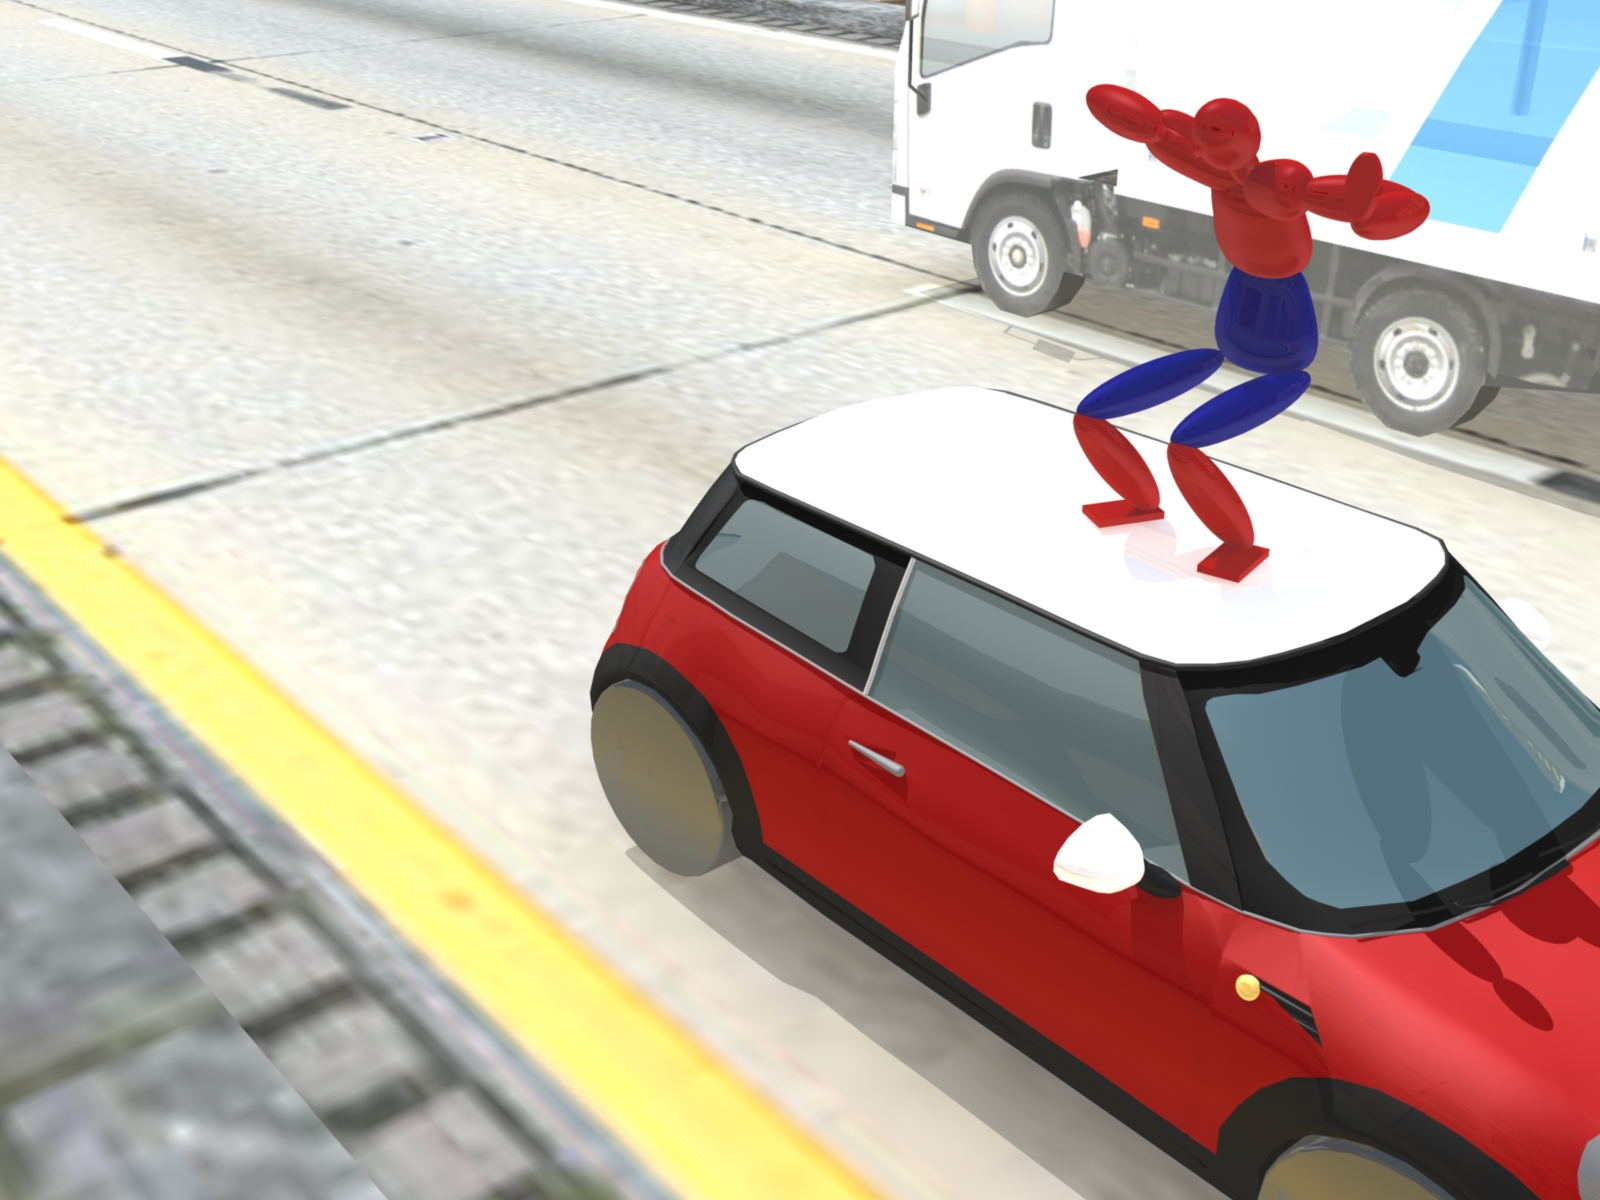
\includegraphics[width=0.48\textwidth]{images/intro_landing.jpg}
  \end{center}
   \vspace{-25pt}
  \caption{A falling motion of Parkour.}
  \label{fig:intro_landing}
   \vspace{-10pt}
\end{wrapfigure}
In Chapter 3, I will show how to create an on-line controller for generating 
agile and natural falling motions of the virtual character that can land from 
various heights and velocities.
The goals of the controller are to reduce the joint stress at the impact and
get back on its feet to prepare the next action.
Inspired by falling skills of Parkour(\figref{intro_landing}), I formulate the falling problem
with three phases, \emph{airborne}, \emph{impact}, and \emph{rolling}
based on the contact states.
First, two sub-controllers are designed for the \emph{airborne} and
\emph{rolling} phases and a regression analysis is conducted to find 
an optimal landing angle that can connect two sub controllers at the
\emph{impact} phase.
I will demonstrate that the motion generated by the proposed controller
induces smaller joint stress, which is still four times lower than a rag-doll
motion at the worst cases.

\subsection{Multiple Contact Planning for Humanoids}
\begin{wrapfigure}{l}{0.5\textwidth}
 \vspace{-25pt}
  \begin{center}
    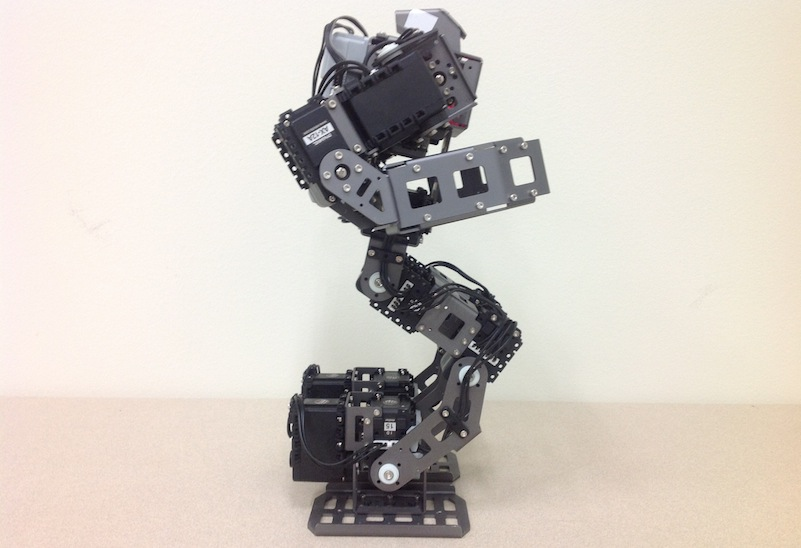
\includegraphics[width=0.48\textwidth]{images/intro_hardware.jpg}
  \end{center}
   \vspace{-25pt}
  \caption{Hardware of BioloidGP robot.}
   \vspace{-10pt}
  \label{fig:intro_hardware}
\end{wrapfigure}
% Goal, Method (Strength), Verification + Image
Chapter 4 will describe a general algorithm which plans for appropriate 
responses to a wide variety of falls, from a single step to recover a gentle nudge, to a rolling motion to break a high-speed fall.
Our multiple contact planning provides a unified framework
that can represent many existing falling techniques [,,].
Then, I will show how to efficiently optimize the multiple contact falling
strategy to the given initial state using a simplified model and dynamic 
programming.
Finally, various scenarios will be tested on simulated humanoids and the
actual hardware (\figref{intro_hardware}) to show that our algorithm plans
various falling strategies with different contact sequences.

\section{Learning of Dynamic Controller for Characters}
% Introduction on the learning - Motivation, Description, Goal
Teaching a physically simulated character a new motor skill requires 
a lot of efforts from the controller designer, from the design of the control 
mechanism to the tweaking of low-level control parameters.
To simplify the learning process, I will introduce an intuitive and 
interactive framework for developing dynamic controllers that is inspired by
how humans learn dynamic motor skills through a iterative process of coaching
and practicing.
Further, we propose two optimization techniques that can extend the popular
policy search algorithm, CMA-ES, to accelerate the convergence rate
and to optimize a parametrized objective function.

\subsection{Iterative Design of Dynamic Controllers}
% Goal, Method (Strength), Verification + Image
\begin{wrapfigure}{r}{0.6\textwidth}
 \vspace{-10pt}
  \begin{center}
    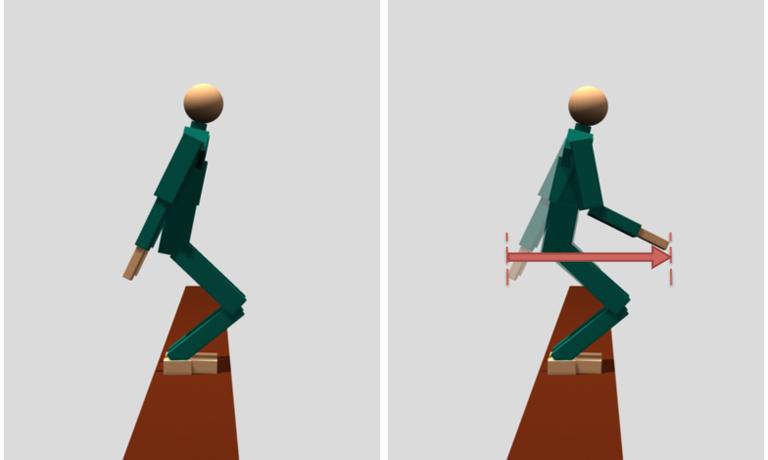
\includegraphics[width=0.58\textwidth]{images/intro_teach.png}
  \end{center}
   \vspace{-25pt}
  \caption{The proposed learning frame uses human readable instructions
    to teach motions.}
  \label{fig:intro_teach}
   \vspace{-10pt}
\end{wrapfigure}
In Chapter 5, I will describe an iterative framework to design dynamic
controllers using high-level, human-readable instructions,
inspired by a training process of athletes that consists of
interactive coaching and repetitive practices (\figref{intro_teach})
To enable interactive coaching, I introduce ``control rigs'' as
an intermediate layer of control module to facilitate the mapping between
human instructions and low-level control parameters.
During the practicing stage, control parameters are efficiently determined
using CMA-ES, which will be further improved in the following chapters.
The details of controllers development process using our iterative learning
framework will be shown with example parkour motions.

\subsection{Optimization with Failure Learning}
% Goal, Method (Strength), Verification + Image
A controller with many user constraints is difficult to optimize due to the
relatively small feasible region.
In Chapter 6, I will describe a new optimization algorithm based on the
observation of human’s ability to learn from failure.
The proposed algorithm, CMA-C (Covariance Matrix Adaptation with
Classification) utilizes the failed simulation trials to approximate 
an infeasible region in the space of control rig parameters, resulting a
faster convergence than the standard CMA-ES.

\subsection{Optimization for Parametrized Motor Skills}
% Goal, Method (Strength), Verification + Image
In Chapter 7, I will show how to optimize parametrized motor skills that are
essential for autonomous robots operating in an unpredictable environment. 
By evolving a parametrized probability distribution, the algorithm reduces 
the number of samples required to optimize a parametrized skill for 
all the tasks in the range of interest. 

\section{Model-based Learning for virtual and real characters}
% Introduction on the bias

\section{Contributions}
The control and optimization methods discussed in this dissertation provide
several contributions to the computer animation community. 
These contributions are as follows:


\begin{itemize}
\item \textbf{A falling and landing strategy for various initial conditions}
  The algorithm presented in the dissertation allows the character to fall from 
  a wide range of heights and initial speeds, continuously roll on the ground, 
  and get back on its feet, without inducing large stress on joints at any
  moment.
\item \textbf{A multiple contact falling strategy for humanoids}
  We introduce a new planning algorithm to minimize the damage of humanoid 
  falls by utilizing multiple contact points. 
\item \textbf{An iterative learning framework for dynamic motor skills}
  Inspired by how humans learn dynamic motor skills through progressive process 
  of coaching and practices, we introduce an intuitive and interactive 
  framework for developing dynamic controllers. 
\item \textbf{An optimization technique that utilized failed samples}
  We introduce a novel efficient optimization algorithm, CMA-C, that shows 
  that faster convergence rate by approximating the infeasible region of a  
  particular type of failure with Supported Vector Machines.
\item \textbf{An optimization technique for parametrized objectives}
  We introduces an efficient evolutionary optimization algorithm for learning
  parametrized skills to achieve whole-body dynamic tasks. 
\end{itemize}



%% Every dissertation should have an introduction.  You might not realize
%% it, but the introduction should introduce the concepts, backgrouand,
%% and goals of the dissertation.

%% \section{Concepts}

%% This is where we talk about the concepts behind the dissertation.

%% \subsection{Primary Concept}

%% This is the primary concept.

%% \subsection{Secondary Concept}

%% This is the secondary concept.

%% \subsubsection{Even more secondary}

%% This is really not all that important.

%% \begin{table}
%% \caption{A table, centered.}
%% \begin{center}
%% \begin{tabular}{|l|r|}
%%   \hline 
%% Title & Author \\
%% \hline
%% War And Peace & Leo Tolstoy \\
%% The Great Gatsby & F. Scott Fitzgerald \\ \hline
%% \end{tabular}
%% \end{center}
%% \end{table}
%% %%
%% \chapter{Previous Work}

%% Some other research was once performed.

%% \begin{figure}
%% \caption{A first figure.}
%% \end{figure}

%% \begin{figure}
%% \caption{A second figure.}
%% \end{figure}
%% %%
%% \chapter{Conclusion}

\nocite{*}
%% We need this since this file doesn't ACTUALLY \cite anything...
%%
\appendix
\chapter{Some Ancillary Stuff}

Ancillary material should be put in appendices, which 
appear just before the bibliography. 

\begin{postliminary}
\references
\postfacesection{Index}{%
%%             ... generate an index here
%%         look into gatech-thesis-index.sty
}
\begin{vita}
Perry H. Disdainful was born in an insignificant town
whose only claim to fame is that it produced such a fine
specimen of a researcher.
\end{vita}
\end{postliminary}

\begin{abstract}
  This is the abstract that must be turned in as hard copy to the
  thesis office to meet the UMI requirements. It should \emph{not} be
  included when submitting your ETD. Comment out the abstract
  environment before submitting. It is recommended that you simply
  copy and paste the text you put in the summary environment into this
  environment. The title, your name, the page count, and your
  advisor's name will all be generated automatically.
\end{abstract}

\end{document}
